\chapter{Implementation}
This chapter explores the development phase of the simulator following the outlined design structure. The implementation of the project took place in iterations in order to prioritize features and to decrease the overall complexity of implementing all the requirements at once. The complete source code can be found in Appendix \ref{appendix:code}. Appendix \ref{appendix:userguide} explains how to use the simulation tool, and Appending \ref{appendix:setupguide} explains how to run the code locally.


\section{Introducing used Technologies}
This section is an overview of the technologies implemented during the project so as to give a brief introduction of which library or framework has been employed for each part of the architecture.


\subsection{Node.js}
Node.js is JavaScript framework to create servers. It supports useful features such as asynchronous Input/Output, and real-time communication. The ecosystem of this language is the largest collections of open source libraries in the world, called modules. It has been chosen for the simulator because it is specifically designed to create web applications and it has modules for real-time communication and cryptography functions that are the main functionalities needed for the simulation. In addition, it unifies the application with a single main programming language as JavaScript is used both for back-end and front-end development. 


\subsection{Socket.io}
Socket.io is a real-time library for bi-directional communication between clients and servers. The availability of this library only in JavaScript was one of the main reasons to choose Node.js as the preferred server-side environment. This library is based on web sockets, a communication protocol, and it serves as a high-level wrapper to them.

The communication is event-based. Therefore, the some action needs to happen in order to trigger the execution of some code usually stored in an 'event handler' function.
The ease of use of this library makes it easy to create a real-time applications allowing the effort of development to be focused on the security properties that the simulation needs to achieve, rather than being slowed down by how to create a distributed system and exchange messages with low latency.

The library can be used both on the back-end and front-end, so a client and a server can use the same functions (from the API) to trigger or handle events.


\subsection{React.js}
This is another JavaScript library that allows modular development of graphical user interfaces (GUI) in the form of 'components' that can be reused. It is a uncomplicated to create an interface that are interactive and change aspect based on the state of the application.

Therefore, it is a very handy library to create this simulation tool, to create a self-explanatory GUI that will be updated at each stage of the protocol execution.

React.js is used in conjunction with JSX, a special syntax to describe what the UI should look like based on the logic state of the application/component, which is a mixture of HTML and JavaScript.

Since JSX is a special syntax that needs to be 'transpiled' into plain JavaScript and HTML that the browser can understand. In order to do, 'Babel' transpiler will be used through in conjunction with a module bundler technology called 'Webpack'. This latter simply merge together several components created during the development phase into a unique 'bundle' file that will be sent to the browser.

Indeed, the set up for this library is not straightforward, but it is a valuable asset in building a state-based UI.

\subsection{Other third-parties Libraries}
The following are other libraries utilized for significant functionalities of the system that helped both in terms of functionalities and sped up the development phase.

\subsubsection{Cryptographically Secure Pseudo-Random Number Generator (csprng)} \label{sec:csprng}
A pivotal code functionality to be implemented successfully is a random generator that produces cryptographically secure numbers to be used as secret keys for each adjacency. A generator that provides this property means that each number is equally likely to be generated, preventing any sort of attack based on the statistical frequency of a stream of generated numbers. 
For this reason, the 'random-number-csprng' library has been implemented, where possible, instead of writing functions that manually generate a random number in a given range.

\subsubsection{Random Name Generator}
The final application will support an arbitrary number of participants connected to the application. In order to identify them among each other a Node library to generate random names has been implemented called 'node-random-name'. 

\subsubsection{Mocha \& Chai}
An important aspect for a mature application is to employ a framework for unit-testing, which is a method to prove the correctness of the logic of an application by verifying the output of a unit being tested is indeed what was expected.

In order to do so in this application, the testing frameworks used is Mocha in conjunction with the assertion library Chai. 


\section{Development Approach}
The approach used throughout the project is a lean methodology that consists in brief iterations of design, implementation and testing. This allowed flexibility to review direction and aims of the initial proposal during project evolution. In addition, making use of iterations helped to be mindful of the time and resource constraints that, as in any other project, were present. Namely, iterations assisted the prioritization of which aspects were more important and what were the dependencies between features to arrange their execution sensibly. This approach lead to the division of the requirements in basic and advanced.


The implementation of functionalities progressed in the following order:
\begin{enumerate}
    \item Implement hard-coded version of the protocol in a single JavaScript file with three participants represented by variables and using a general number random generator;
    \item Develop Node.js web application integrated with React.js and transpiling pipeline of Webpack and Babel;
    \item Integrate Socket.io with React.js for real-time communication;
    \item Distribute the execution of basic protocol between clients and server. Each client possess logic functions inside the main React component (AppComponent). The server generates adjacencies and reacts to events such as connection and disconnection of a client which may trigger the start of the protocol;
    \item Substitute simple random generator with a cryptographically secure pseudo-random number generator;
    \item Implement random name generator to have unique client names;
    \item Introduce objects (Adjacency, Participant, Round) to group functionalities and attributes together and improve modularity of the codebase;
    \item Implement security mechanism to abort communication with less than 3 clients;
    \item Implement clean-up functionalities for the client's browser. This clears keys and other local data when communication is aborted but then restarts again;
    \item Refactor code after having implemented all of the basic features, separating, where possible, the logic of the protocol from the sever-client communication functions;
    \item Implement helper messages on hover for the main steps of the protocol execution;
    \item Start Unit-Testing of the logic functions;
    \item Refactor the AppComponent into smaller React components, each responsible for a single element of the GUI;
    \item deploy application 
    \item Repeat protocol execution continuously, so as to have multiple rounds of communication;
    \item Support connection of an arbitrary number of clients to the server;
    \item Handle connection and disconnection of clients in the middle of round execution;
    \item Implement key storage on the server and utilize this to detect collision;
    \item Implement 8-bit keys;
    \item Divide communication into three types of rounds (voting round, length-calculation round, communication round) and all the relative features that this division entails;
    \item Implement the new security mechanisms needed: prevent the message sender to win the next voting round; abort round when message sender disconnects during round; abort communication if all clients try to send a message in the same round;
    \item Refine user-interface to improve user-friendliness and perform final refactor of codebase;
\end{enumerate}


\subsection{Development Pipeline Tools}
To publish the simulator online, a continuous integration development pipeline was created. This simply means that new features are available live as soon as the codebase updates happen, ensuring that the application is tested correctly. \newline

Firstly, the code is uploaded on Github, a code-sharing platform where a user can store projects.

Secondly, through the presence of a webhook on Github, a code update will trigger the automatic execution of unit-tests in Circle CI (continuous integration). This ensures that new features did not break functionalities previously built.

Lastly, If all tests successful the code is automatically released on the web hosting platform Heroku. The application is in fact available at \url{https://www.dc-net.herokuapp.com}.

\begin{figure}[h!]
    \centering
    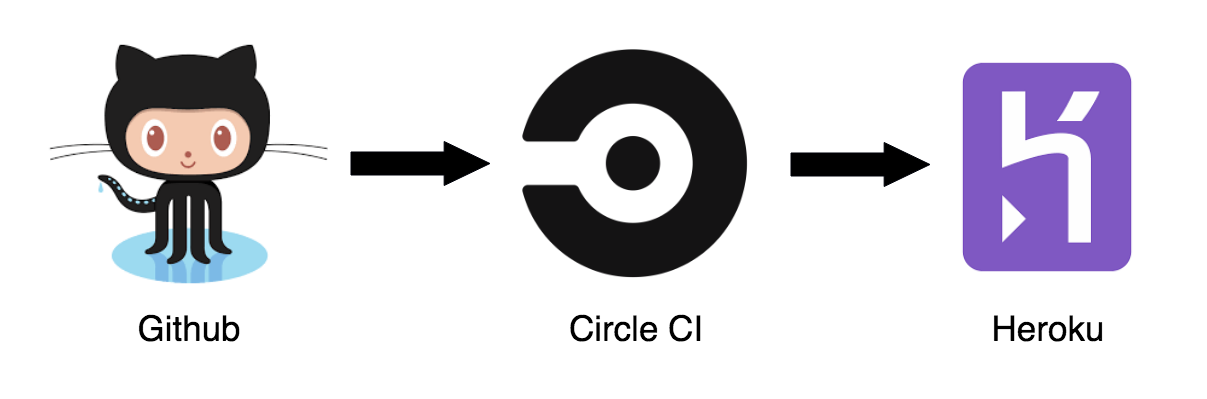
\includegraphics[width=0.70\textwidth]{Images/pipeline.png}
    \caption{Development Pipeline}
    \label{fig:devPipeline}
\end{figure}


\section{Basic Implemented System}
This section presents the main components of the simulator implemented at the completion of the basic requirements. 

\emph{Please note that all the features presented are implemented in the code. However, some of the code snippets presented in this section are not exactly the same as in the source code, since the version provided in the appendix is the final product that also includes the advanced requirements.}

\subsection{Initial Connection} \label{sec:initialConnection}
A client that connects to the server, by typing \lstinline{https://www.dc-net.herokuapp.com} in his browser, will automatically trigger a socket \lstinline{connection} event. This turns the simple \lstinline{HTTP get} request of the page into a \lstinline{TCP} session. This happens thanks to a \lstinline{HTTP Upgrade} request. The result is a stable open connection between a client and a server, and both ends listen to incoming \lstinline{socket.io} events.


\subsection{Socket.io communication example}
\lstinline{Socket.io} provides an API that is used by the server to trigger, i.e. emit, real-time events that will instantly reach the client/clients. The following are two examples of \lstinline{emit} events: 

\begin{lstlisting}
  /* server sends broadcast event 'client-connection' to all connected clients and sends them the name of the participant that just connected*/
  io.sockets.emit('client-connection', newParticipant.name);
  
  /* server sends unicast event 'client-connection' to client1 with the name of the name of the participant that just connected */
  io.sockets.to(client1.id).emit('client-connection', newParticipant.name);
\end{lstlisting}

The first parameter of the emit function is always the event name, and the optional following parameters are the data being sent. \newline

In order for a client to handle an event emitted by the server the function \lstinline{socket.on('event-name')} is employed. A small API to combine React.js and Socket.io was created (source code file \lstinline{socket-api.js}). Each function developed is a wrapper function that receives a callback as a parameter to be invoked when the specific socket event is received by the sever. For Example: 
\begin{lstlisting}
    // example of wrapper function to socket.on event.
    function connectionEvent(callback) {
        /* client socket listens to 'client-connection' event. When receiving this event a single paramenter 'name' is expected */
        socket.on('client-connection', (name) => {
                // invoking function that was passed as a parameter
                callback(name);
            }
        );
    }
\end{lstlisting}

The client provides the callback parameter for a socket event in the React.js component called \lstinline{AppComponent}. In fact, only the \lstinline{AppComponent} in the developed application will interact with socket events, so that there exist a centralized place to communicate with the back-end. The \lstinline{socket-api.js} functions are imported in the \lstinline{AppComponent} and, following the example above, the callback to the \lstinline{connectionEvent} function can be provided as follows: 
\begin{lstlisting}
    /* connectionEvent function called with an arrow function as parameter, which is the callback that will be invoked when the socket event 'client-connection' will be received */
    connectionEvent((name) => {
        /* update state of AppComponent adding a connection object to the list of events */
        this.setState({
            events: [...this.state.events, new Connection(name)],
        });
    });
\end{lstlisting}

In the same way, a client can emit an event with \lstinline{socket.emit('event-name1');} and this will be received by the server. If the this latter has a corresponding \lstinline|socket.on('event-name1', () => { /* do something on the server */  });| then, an action is triggered. \newline


To summarize, all the exchanges between the server and the client, with exception of the initial \lstinline{HTTP get} request, will take place through \lstinline{socket.io} real-time library. Both the server and clients can emit and listen to events, and perform some computation accordingly. 


\subsection{State of Client \& UI updates}
React.js front-end components can have their own state. This is simply an object where information of that component is stored.
\begin{lstlisting}
    // state object example of basic implementation. A state can be intialized in the constructor of the React component.
    this.state = {
        events: [],
        showDiagol: false,
        roundNumber: 0,
        roundInProgress: false,
        whoami: '',
    };
    
    // example command to access the roundNumber variable of the state
    this.state.roundNumber;
    
    /* how to update state. Need to use setState() function cannot change state variables directly */
    this.setState({
        roundNumber: ++roundNumber;
    });
\end{lstlisting}

The React.js feature that updates the user interface is the automatic re-rendering triggered when \lstinline{this.setState()} function is invoked.

This is a simple yet powerful concept that allows a granular manipulation of the interface.


\subsection{Trigger execution of the protocol}
The server starts of the execution of the protocol as soon as three clients establish a connection. This is possible because, as mentioned in section \ref{sec:initialConnection}, a \lstinline{connection} event is emitted by the client at connection time and received by the server. The basic version of the connectionHandler on the server creates a new Participant objects and stores it in a list to keep track of the current connections, it broadcasts to all clients the fact that a new connection happened, and if at least three users are connected the protocol begins.

\begin{lstlisting}
    // handle a new client connection on connection on the server.
    function handleNewConnection(socket) {
        var newParticipant = new Participant(generateUniqueRandomName(participants), socket.id);
        participants = [...participants, newParticipant];
        broadcastEvent('client-connection', newParticipant.name);
        if (participants.length == 3) {
            // start protocol execution
            beginCommunication();
        } else if (participants.length > 3) {
            // basic implementation supported only three participants
            throw new Error ("too many participants connected");
        }
    };
\end{lstlisting}


\subsection{Generating Adjacencies}
Another fundamental part of the protocol is to generate a neighbouring relationships between pairs of clients. This step is important so that the server can generate a secret key for each adjacency. 

\begin{lstlisting}
    function generateAdjacencies(participants) {
        let adjacencies = [];
        for (var x = 0; x < participants.length; ++x) {
            var current = x;
            var next = (x + 1) \% participants.length;
            // create new Adjacency object with two clients.
            var adj = new Adjacency(participants[current], participants[next]);
            // add the new object to the list of created adjacencies so far
            adjacencies = [...adjacencies, adj];
        }
        return adjacencies;
    }
\end{lstlisting}

\subsection{Generating secure random numbers as secret keys}
The random generation of secure keys is crucial to ensure untraceability of the protocol. As mentioned in section \ref{sec:csprng}, a third party library was employed. Since it may take few moments to generate such number, the numer is generated asynchronously. Therefore, a wrapper function has been built to then employ it where it is needed.

\begin{lstlisting}
    function csprnGenerator(minimum, maximum, callback) {
        Promise.try(function() {
            // create random number in range
            return randomNumber(minimum, maximum);
        }).then(function(secureRandom) {
            // invoke callback passing the secure random number as a parameter
            callback(secureRandom);
        }).catch({code: 'RandomGenerationError'}, function(err) {
            console.error('csprn generation error.');
        });
    }
\end{lstlisting}

\subsection{XOR functions}
Once the keys have been generated from the server and received by the clients, the main logic operation of the protocol takes place: XOR of secret keys and, in case of the message sender, participant message. In the basic version of the protocol the client can simply express the intention to send a message. 'Yes' equates to XORing the secret keys with 1, and 'No' equates to XORing the secret keys with 0.

The XOR operation in JavaScript is called 'Bitwise XOR Operator' \cite{XORJS} and its symbol is $\wedge$.
\begin{lstlisting}
    // XOR function on the browser's client
    calculateXORValue(key1, key2, participantMessage) {
        return key1 ^ key2 ^ participantMessage;
    }
\end{lstlisting}

The responses of the clients are sent to the server. These messages could even be transmitted in plain text, since being aware of all participant responses does not reveal any information about who the sender is. \newline

Once all the results reach the server, its role is to combine them so as to reveal what the anonymous round message is, which will then broadcasted to all participants in the network. A function for the class Round was created, and it is invoked a static function.

\begin{lstlisting}
    Round.prototype.calculateXORRoundResult = function(participants) {
        let roundResult = 0;
        // XOR all rounds messages together
        for(var x=0; x < participants.length; ++x) {
            roundResult ^= participants[x].roundMessage;
        }
        return roundResult;
    }
\end{lstlisting}


\subsection{A round of communication}
Using the logic components, the most important of which were presented above, jointly with socket.io events the protocol is successfully carried out.

\begin{figure}[H]
    \centering
    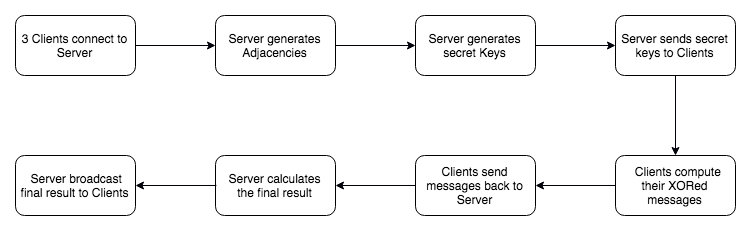
\includegraphics[width=1\textwidth]{Images/Implementation/protocolExecuted.png}
    \caption{Main steps of protocol execution}
    \label{fig:protocolExecuted}
\end{figure}

Beside the main steps described and presented in figure \ref{fig:protocolExecuted}, there are more underlying \lstinline{socket.io} events communicated in order to update the graphical user interface of the user and provide explicate content about each stage of the protocol.

\section{Advanced Implemented System}
This sections presents the more complex system achieved at the end of the project with the implementation of all of the advanced requirements.



\subsection{Collision Detection}

\subsection{Handle Connections and Disconnections}

\subsubsection{Browser Connections Limit}

\subsection{Arbitrary number of participants}


\section{Unit Testing}
As previously mentioned, unit testing is the execution of tests on small parts of the codebase, usually one function at a time. This happens by running a given function with some chosen input and comparing the expected output with the actual output. 

Not only unit testing has the main purpose of checking the correct execution of the logic of your application, but it also helps to break down the codebase into separate functions, each one with its specific purpose, since it would otherwise be difficult to test.



\section{Implementation roadblocks}


\section{Mapping Theoretical Concepts to Implementation}